\documentclass{amsart}
\usepackage{amsmath}
\usepackage{amssymb}
\usepackage{tikz}
\usepackage[utf8]{inputenc}
\usepackage{pgfplots}
\usepackage{color}
\usetikzlibrary{decorations.markings}
\usetikzlibrary{arrows.meta}

\begin{document}

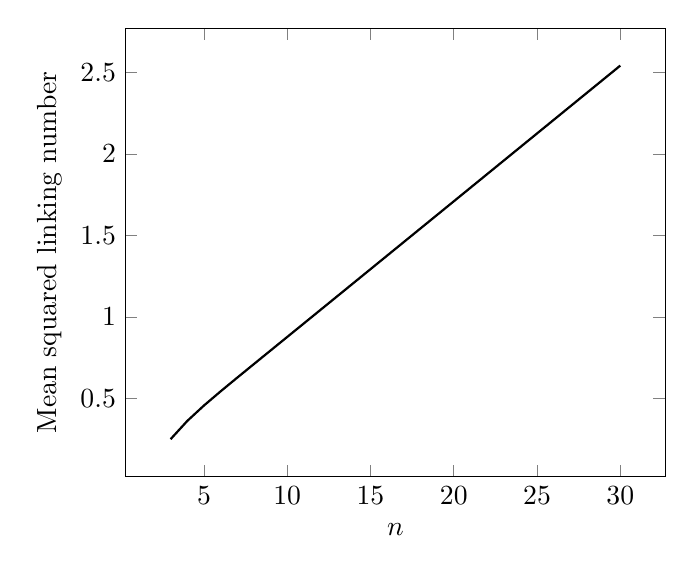
\begin{tikzpicture} \begin{axis}[ xlabel=$n$, ylabel=Mean squared linking number ]

		\addplot[thick,color=black] coordinates { (3,1/4) (4,38/105) (5,115/252)
		(6,251/462) (7,497/792) (8,13724/19305) (9,2271/2860) (10,243095/277134)
		(11,677435/705432) (12,705431/676039) (13,2343601/2080120) 
		(20,35345263799/20676979323) (30,150336332497705195/59132290782430712)};

		\end{axis} \end{tikzpicture}

\end{document}